% Benötigt in der Präambel: \usepackage{pgfplots}
% und \pgfplotsset{compat=1.18}.
% Diese Datei und kapitel5-ergebnisse.tex in denselben Ordner legen.
% Beim Einbinden aus einem Unterordner den folgenden Eingabepfad anpassen.
% Generated by npm run evaluate; experiment selection-benchmark-v6-longitudinal.
\newcommand{\EvaluationSessions}{5985}
\newcommand{\EvaluationAnswers}{172088}
\newcommand{\EvaluationEvidenceEnds}{58}
\newcommand{\EvaluationNoQuestionEnds}{342}
\newcommand{\EvaluationBrierTable}{%
\begin{tabular}{llccc}
\hline
Situation & Sitzung & Zufall & Bewertungen + Lernstand & Informationsgewinn \\
\hline
Niedrig & 1 & \shortstack{$0{,}2294 \pm 0{,}0178$\\(0{,}2319)} & \shortstack{$0{,}2331 \pm 0{,}0226$\\(0{,}2347)} & \shortstack{$0{,}2346 \pm 0{,}0192$\\(0{,}2370)} \\
Niedrig & 2 & \shortstack{$0{,}2236 \pm 0{,}0271$\\(0{,}2416)} & \shortstack{$0{,}2313 \pm 0{,}0243$\\(0{,}2388)} & \shortstack{$0{,}2340 \pm 0{,}0217$\\(0{,}2380)} \\
Niedrig & 3 & \shortstack{$0{,}2195 \pm 0{,}0286$\\(0{,}2501)} & \shortstack{$0{,}2344 \pm 0{,}0261$\\(0{,}2411)} & \shortstack{$0{,}2334 \pm 0{,}0199$\\(0{,}2411)} \\
Niedrig & 4 & \shortstack{$0{,}2016 \pm 0{,}0368$\\(0{,}2571)} & \shortstack{$0{,}2341 \pm 0{,}0287$\\(0{,}2434)} & \shortstack{$0{,}2310 \pm 0{,}0288$\\(0{,}2443)} \\
Niedrig & 5 & \shortstack{$0{,}1945 \pm 0{,}0439$\\(0{,}2622)} & \shortstack{$0{,}2308 \pm 0{,}0270$\\(0{,}2454)} & \shortstack{$0{,}2309 \pm 0{,}0280$\\(0{,}2485)} \\
Gemischt & 1 & \shortstack{$0{,}2366 \pm 0{,}0187$\\(0{,}2499)} & \shortstack{$0{,}2343 \pm 0{,}0224$\\(0{,}2501)} & \shortstack{$0{,}2329 \pm 0{,}0179$\\(0{,}2519)} \\
Gemischt & 2 & \shortstack{$0{,}2117 \pm 0{,}0258$\\(0{,}2572)} & \shortstack{$0{,}2322 \pm 0{,}0223$\\(0{,}2527)} & \shortstack{$0{,}2322 \pm 0{,}0215$\\(0{,}2506)} \\
Gemischt & 3 & \shortstack{$0{,}1994 \pm 0{,}0308$\\(0{,}2633)} & \shortstack{$0{,}2330 \pm 0{,}0243$\\(0{,}2493)} & \shortstack{$0{,}2303 \pm 0{,}0217$\\(0{,}2522)} \\
Gemischt & 4 & \shortstack{$0{,}1771 \pm 0{,}0399$\\(0{,}2695)} & \shortstack{$0{,}2288 \pm 0{,}0250$\\(0{,}2492)} & \shortstack{$0{,}2271 \pm 0{,}0278$\\(0{,}2514)} \\
Gemischt & 5 & \shortstack{$0{,}1695 \pm 0{,}0435$\\(0{,}2718)} & \shortstack{$0{,}2259 \pm 0{,}0253$\\(0{,}2501)} & \shortstack{$0{,}2289 \pm 0{,}0293$\\(0{,}2498)} \\
Hoch & 1 & \shortstack{$0{,}2486 \pm 0{,}0187$\\(0{,}2861)} & \shortstack{$0{,}2266 \pm 0{,}0173$\\(0{,}2852)} & \shortstack{$0{,}2322 \pm 0{,}0186$\\(0{,}2845)} \\
Hoch & 2 & \shortstack{$0{,}1862 \pm 0{,}0280$\\(0{,}2884)} & \shortstack{$0{,}2281 \pm 0{,}0185$\\(0{,}2832)} & \shortstack{$0{,}2235 \pm 0{,}0153$\\(0{,}2850)} \\
Hoch & 3 & \shortstack{$0{,}1546 \pm 0{,}0385$\\(0{,}2887)} & \shortstack{$0{,}2195 \pm 0{,}0170$\\(0{,}2805)} & \shortstack{$0{,}2162 \pm 0{,}0193$\\(0{,}2827)} \\
Hoch & 4 & \shortstack{$0{,}1272 \pm 0{,}0418$\\(0{,}2913)} & \shortstack{$0{,}1979 \pm 0{,}0374$\\(0{,}2733)} & \shortstack{$0{,}2065 \pm 0{,}0423$\\(0{,}2679)} \\
Hoch & 5 & \shortstack{$0{,}1193 \pm 0{,}0461$\\(0{,}2922)} & \shortstack{$0{,}2269 \pm 0{,}0763_{n=89}$\\(0{,}2622)} & \shortstack{$0{,}1981 \pm 0{,}0785_{n=96}$\\(0{,}2635)} \\
Abweichend & 1 & \shortstack{$0{,}2478 \pm 0{,}0225$\\(0{,}2507)} & \shortstack{$0{,}2462 \pm 0{,}0279$\\(0{,}2484)} & \shortstack{$0{,}2468 \pm 0{,}0216$\\(0{,}2511)} \\
Abweichend & 2 & \shortstack{$0{,}2467 \pm 0{,}0283$\\(0{,}2531)} & \shortstack{$0{,}2487 \pm 0{,}0268$\\(0{,}2499)} & \shortstack{$0{,}2488 \pm 0{,}0293$\\(0{,}2482)} \\
Abweichend & 3 & \shortstack{$0{,}2465 \pm 0{,}0426$\\(0{,}2536)} & \shortstack{$0{,}2446 \pm 0{,}0314$\\(0{,}2468)} & \shortstack{$0{,}2488 \pm 0{,}0274$\\(0{,}2486)} \\
Abweichend & 4 & \shortstack{$0{,}2423 \pm 0{,}0406$\\(0{,}2555)} & \shortstack{$0{,}2505 \pm 0{,}0267$\\(0{,}2436)} & \shortstack{$0{,}2529 \pm 0{,}0333$\\(0{,}2463)} \\
Abweichend & 5 & \shortstack{$0{,}2345 \pm 0{,}0432$\\(0{,}2566)} & \shortstack{$0{,}2454 \pm 0{,}0303$\\(0{,}2443)} & \shortstack{$0{,}2447 \pm 0{,}0301$\\(0{,}2404)} \\
\hline
\end{tabular}}
\newcommand{\EvaluationLogLossTable}{%
\begin{tabular}{llccc}
\hline
Situation & Sitzung & Zufall & Bewertungen + Lernstand & Informationsgewinn \\
\hline
Niedrig & 1 & \shortstack{$0{,}6521 \pm 0{,}0382$\\(0{,}6567)} & \shortstack{$0{,}6601 \pm 0{,}0474$\\(0{,}6625)} & \shortstack{$0{,}6630 \pm 0{,}0402$\\(0{,}6671)} \\
Niedrig & 2 & \shortstack{$0{,}6388 \pm 0{,}0604$\\(0{,}6763)} & \shortstack{$0{,}6561 \pm 0{,}0507$\\(0{,}6707)} & \shortstack{$0{,}6618 \pm 0{,}0455$\\(0{,}6690)} \\
Niedrig & 3 & \shortstack{$0{,}6292 \pm 0{,}0659$\\(0{,}6933)} & \shortstack{$0{,}6621 \pm 0{,}0542$\\(0{,}6754)} & \shortstack{$0{,}6605 \pm 0{,}0416$\\(0{,}6754)} \\
Niedrig & 4 & \shortstack{$0{,}5849 \pm 0{,}0854$\\(0{,}7073)} & \shortstack{$0{,}6616 \pm 0{,}0596$\\(0{,}6799)} & \shortstack{$0{,}6553 \pm 0{,}0600$\\(0{,}6817)} \\
Niedrig & 5 & \shortstack{$0{,}5728 \pm 0{,}1070$\\(0{,}7176)} & \shortstack{$0{,}6544 \pm 0{,}0560$\\(0{,}6838)} & \shortstack{$0{,}6544 \pm 0{,}0581$\\(0{,}6901)} \\
Gemischt & 1 & \shortstack{$0{,}6651 \pm 0{,}0401$\\(0{,}6930)} & \shortstack{$0{,}6611 \pm 0{,}0474$\\(0{,}6933)} & \shortstack{$0{,}6578 \pm 0{,}0376$\\(0{,}6970)} \\
Gemischt & 2 & \shortstack{$0{,}6103 \pm 0{,}0594$\\(0{,}7076)} & \shortstack{$0{,}6564 \pm 0{,}0467$\\(0{,}6985)} & \shortstack{$0{,}6568 \pm 0{,}0454$\\(0{,}6944)} \\
Gemischt & 3 & \shortstack{$0{,}5829 \pm 0{,}0742$\\(0{,}7199)} & \shortstack{$0{,}6585 \pm 0{,}0509$\\(0{,}6917)} & \shortstack{$0{,}6529 \pm 0{,}0454$\\(0{,}6976)} \\
Gemischt & 4 & \shortstack{$0{,}5276 \pm 0{,}0953$\\(0{,}7322)} & \shortstack{$0{,}6498 \pm 0{,}0522$\\(0{,}6916)} & \shortstack{$0{,}6459 \pm 0{,}0582$\\(0{,}6961)} \\
Gemischt & 5 & \shortstack{$0{,}5133 \pm 0{,}1089$\\(0{,}7369)} & \shortstack{$0{,}6436 \pm 0{,}0526$\\(0{,}6933)} & \shortstack{$0{,}6500 \pm 0{,}0607$\\(0{,}6927)} \\
Hoch & 1 & \shortstack{$0{,}6863 \pm 0{,}0412$\\(0{,}7656)} & \shortstack{$0{,}6413 \pm 0{,}0370$\\(0{,}7639)} & \shortstack{$0{,}6531 \pm 0{,}0396$\\(0{,}7624)} \\
Hoch & 2 & \shortstack{$0{,}5495 \pm 0{,}0663$\\(0{,}7704)} & \shortstack{$0{,}6448 \pm 0{,}0396$\\(0{,}7598)} & \shortstack{$0{,}6350 \pm 0{,}0327$\\(0{,}7634)} \\
Hoch & 3 & \shortstack{$0{,}4794 \pm 0{,}0958$\\(0{,}7710)} & \shortstack{$0{,}6271 \pm 0{,}0361$\\(0{,}7544)} & \shortstack{$0{,}6199 \pm 0{,}0411$\\(0{,}7588)} \\
Hoch & 4 & \shortstack{$0{,}4115 \pm 0{,}1058$\\(0{,}7761)} & \shortstack{$0{,}5823 \pm 0{,}0795$\\(0{,}7400)} & \shortstack{$0{,}6006 \pm 0{,}0899$\\(0{,}7291)} \\
Hoch & 5 & \shortstack{$0{,}3948 \pm 0{,}1197$\\(0{,}7779)} & \shortstack{$0{,}6460 \pm 0{,}1603_{n=89}$\\(0{,}7176)} & \shortstack{$0{,}5854 \pm 0{,}1660_{n=96}$\\(0{,}7202)} \\
Abweichend & 1 & \shortstack{$0{,}6899 \pm 0{,}0488$\\(0{,}6945)} & \shortstack{$0{,}6865 \pm 0{,}0590$\\(0{,}6900)} & \shortstack{$0{,}6875 \pm 0{,}0456$\\(0{,}6953)} \\
Abweichend & 2 & \shortstack{$0{,}6908 \pm 0{,}0644$\\(0{,}6994)} & \shortstack{$0{,}6916 \pm 0{,}0567$\\(0{,}6930)} & \shortstack{$0{,}6919 \pm 0{,}0619$\\(0{,}6896)} \\
Abweichend & 3 & \shortstack{$0{,}6961 \pm 0{,}1017$\\(0{,}7003)} & \shortstack{$0{,}6831 \pm 0{,}0657$\\(0{,}6866)} & \shortstack{$0{,}6919 \pm 0{,}0576$\\(0{,}6904)} \\
Abweichend & 4 & \shortstack{$0{,}6878 \pm 0{,}1005$\\(0{,}7042)} & \shortstack{$0{,}6955 \pm 0{,}0558$\\(0{,}6803)} & \shortstack{$0{,}7009 \pm 0{,}0700$\\(0{,}6858)} \\
Abweichend & 5 & \shortstack{$0{,}6720 \pm 0{,}1064$\\(0{,}7064)} & \shortstack{$0{,}6850 \pm 0{,}0633$\\(0{,}6816)} & \shortstack{$0{,}6837 \pm 0{,}0633$\\(0{,}6739)} \\
\hline
\end{tabular}}
\newcommand{\EvaluationNeedTable}{%
\begin{tabular}{llccc}
\hline
Situation & Sitzung & Zufall & Bewertungen + Lernstand & Informationsgewinn \\
\hline
Niedrig & 1 & \shortstack{$84{,}3 \pm 6{,}5$} & \shortstack{$79{,}9 \pm 8{,}4$} & \shortstack{$78{,}3 \pm 7{,}9$} \\
Niedrig & 2 & \shortstack{$71{,}9 \pm 9{,}3$} & \shortstack{$76{,}3 \pm 9{,}2$} & \shortstack{$76{,}8 \pm 8{,}5$} \\
Niedrig & 3 & \shortstack{$61{,}7 \pm 9{,}0$} & \shortstack{$73{,}8 \pm 9{,}5$} & \shortstack{$73{,}1 \pm 7{,}4$} \\
Niedrig & 4 & \shortstack{$52{,}1 \pm 9{,}1$} & \shortstack{$70{,}9 \pm 10{,}5$} & \shortstack{$68{,}1 \pm 10{,}3$} \\
Niedrig & 5 & \shortstack{$46{,}7 \pm 8{,}7$} & \shortstack{$67{,}9 \pm 10{,}7$} & \shortstack{$64{,}7 \pm 9{,}8$} \\
Gemischt & 1 & \shortstack{$61{,}1 \pm 7{,}5$} & \shortstack{$61{,}5 \pm 10{,}8$} & \shortstack{$58{,}9 \pm 9{,}0$} \\
Gemischt & 2 & \shortstack{$51{,}8 \pm 10{,}2$} & \shortstack{$59{,}4 \pm 9{,}1$} & \shortstack{$60{,}9 \pm 8{,}7$} \\
Gemischt & 3 & \shortstack{$44{,}1 \pm 9{,}1$} & \shortstack{$63{,}0 \pm 10{,}7$} & \shortstack{$58{,}8 \pm 7{,}9$} \\
Gemischt & 4 & \shortstack{$36{,}5 \pm 8{,}7$} & \shortstack{$61{,}9 \pm 12{,}4$} & \shortstack{$60{,}4 \pm 12{,}3$} \\
Gemischt & 5 & \shortstack{$34{,}4 \pm 8{,}0$} & \shortstack{$60{,}7 \pm 11{,}4$} & \shortstack{$62{,}3 \pm 11{,}4$} \\
Hoch & 1 & \shortstack{$14{,}1 \pm 6{,}3$} & \shortstack{$15{,}4 \pm 8{,}5$} & \shortstack{$16{,}5 \pm 6{,}3$} \\
Hoch & 2 & \shortstack{$11{,}5 \pm 5{,}8$} & \shortstack{$17{,}5 \pm 8{,}6$} & \shortstack{$15{,}8 \pm 6{,}6$} \\
Hoch & 3 & \shortstack{$10{,}0 \pm 4{,}6$} & \shortstack{$21{,}2 \pm 10{,}4$} & \shortstack{$18{,}3 \pm 8{,}3$} \\
Hoch & 4 & \shortstack{$8{,}1 \pm 5{,}4$} & \shortstack{$33{,}1 \pm 15{,}9$} & \shortstack{$38{,}4 \pm 17{,}2$} \\
Hoch & 5 & \shortstack{$7{,}0 \pm 5{,}2$} & \shortstack{$46{,}7 \pm 35{,}5_{n=89}$} & \shortstack{$45{,}0 \pm 30{,}8_{n=96}$} \\
Abweichend & 1 & \shortstack{$63{,}7 \pm 7{,}1$} & \shortstack{$66{,}9 \pm 11{,}7$} & \shortstack{$64{,}7 \pm 8{,}1$} \\
Abweichend & 2 & \shortstack{$60{,}5 \pm 9{,}7$} & \shortstack{$67{,}5 \pm 10{,}0$} & \shortstack{$68{,}0 \pm 8{,}0$} \\
Abweichend & 3 & \shortstack{$58{,}4 \pm 9{,}0$} & \shortstack{$71{,}8 \pm 10{,}8$} & \shortstack{$68{,}4 \pm 9{,}0$} \\
Abweichend & 4 & \shortstack{$55{,}0 \pm 10{,}4$} & \shortstack{$76{,}4 \pm 10{,}1$} & \shortstack{$76{,}3 \pm 11{,}2$} \\
Abweichend & 5 & \shortstack{$54{,}8 \pm 10{,}5$} & \shortstack{$79{,}2 \pm 10{,}9$} & \shortstack{$81{,}5 \pm 8{,}9$} \\
\hline
\end{tabular}}
\newcommand{\EvaluationCoverageTable}{%
\begin{tabular}{llccc}
\hline
Situation & Sitzung & Zufall & Bewertungen + Lernstand & Informationsgewinn \\
\hline
Niedrig & 1 & \shortstack{$55{,}4 \pm 4{,}7$} & \shortstack{$29{,}9 \pm 2{,}0$} & \shortstack{$33{,}2 \pm 1{,}0$} \\
Niedrig & 2 & \shortstack{$55{,}5 \pm 4{,}9$} & \shortstack{$30{,}5 \pm 2{,}1$} & \shortstack{$29{,}1 \pm 1{,}8$} \\
Niedrig & 3 & \shortstack{$55{,}8 \pm 4{,}3$} & \shortstack{$31{,}1 \pm 2{,}6$} & \shortstack{$28{,}2 \pm 2{,}7$} \\
Niedrig & 4 & \shortstack{$55{,}9 \pm 4{,}2$} & \shortstack{$32{,}3 \pm 3{,}2$} & \shortstack{$32{,}5 \pm 4{,}0$} \\
Niedrig & 5 & \shortstack{$56{,}2 \pm 4{,}6$} & \shortstack{$32{,}8 \pm 3{,}5$} & \shortstack{$33{,}4 \pm 3{,}5$} \\
Gemischt & 1 & \shortstack{$55{,}4 \pm 4{,}7$} & \shortstack{$31{,}7 \pm 2{,}3$} & \shortstack{$34{,}7 \pm 1{,}5$} \\
Gemischt & 2 & \shortstack{$55{,}5 \pm 4{,}9$} & \shortstack{$32{,}4 \pm 2{,}2$} & \shortstack{$30{,}4 \pm 1{,}9$} \\
Gemischt & 3 & \shortstack{$55{,}8 \pm 4{,}3$} & \shortstack{$32{,}3 \pm 2{,}8$} & \shortstack{$30{,}4 \pm 3{,}2$} \\
Gemischt & 4 & \shortstack{$55{,}9 \pm 4{,}2$} & \shortstack{$33{,}5 \pm 3{,}2$} & \shortstack{$34{,}7 \pm 3{,}8$} \\
Gemischt & 5 & \shortstack{$56{,}2 \pm 4{,}6$} & \shortstack{$33{,}5 \pm 3{,}7$} & \shortstack{$31{,}4 \pm 3{,}0$} \\
Hoch & 1 & \shortstack{$55{,}4 \pm 4{,}7$} & \shortstack{$36{,}4 \pm 2{,}4$} & \shortstack{$38{,}5 \pm 1{,}6$} \\
Hoch & 2 & \shortstack{$55{,}5 \pm 4{,}9$} & \shortstack{$36{,}2 \pm 2{,}4$} & \shortstack{$34{,}8 \pm 1{,}8$} \\
Hoch & 3 & \shortstack{$55{,}8 \pm 4{,}3$} & \shortstack{$37{,}0 \pm 2{,}8$} & \shortstack{$36{,}7 \pm 3{,}7$} \\
Hoch & 4 & \shortstack{$55{,}9 \pm 4{,}2$} & \shortstack{$23{,}3 \pm 6{,}6$} & \shortstack{$20{,}7 \pm 6{,}6$} \\
Hoch & 5 & \shortstack{$56{,}2 \pm 4{,}6$} & \shortstack{$6{,}3 \pm 2{,}9_{n=89}$} & \shortstack{$6{,}4 \pm 3{,}0_{n=96}$} \\
Abweichend & 1 & \shortstack{$55{,}4 \pm 4{,}7$} & \shortstack{$31{,}3 \pm 2{,}2$} & \shortstack{$34{,}5 \pm 1{,}4$} \\
Abweichend & 2 & \shortstack{$55{,}5 \pm 4{,}9$} & \shortstack{$31{,}4 \pm 2{,}5$} & \shortstack{$29{,}8 \pm 1{,}9$} \\
Abweichend & 3 & \shortstack{$55{,}8 \pm 4{,}3$} & \shortstack{$31{,}7 \pm 2{,}9$} & \shortstack{$29{,}5 \pm 2{,}7$} \\
Abweichend & 4 & \shortstack{$55{,}9 \pm 4{,}2$} & \shortstack{$31{,}5 \pm 2{,}7$} & \shortstack{$31{,}5 \pm 4{,}2$} \\
Abweichend & 5 & \shortstack{$56{,}2 \pm 4{,}6$} & \shortstack{$32{,}6 \pm 3{,}4$} & \shortstack{$31{,}5 \pm 4{,}1$} \\
\hline
\end{tabular}}
\newcommand{\EvaluationBrierPlot}{%
\begin{minipage}{0.48\textwidth}\centering
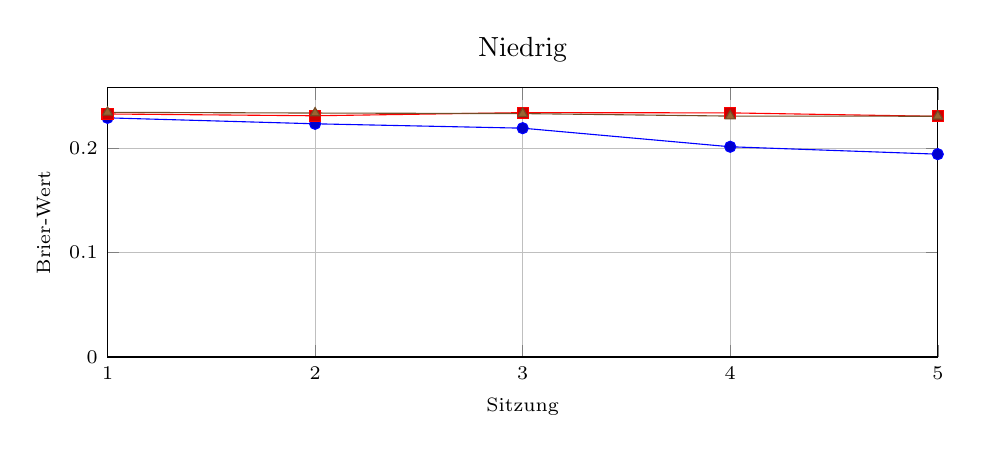
\begin{tikzpicture}
\begin{axis}[width=\linewidth,height=5cm,title={Niedrig},xlabel={Sitzung},ylabel={Brier-Wert},xmin=1,xmax=5,xtick={1,...,5},ymin=0,grid=major,tick label style={font=\scriptsize},label style={font=\scriptsize}]
\addplot+[mark=*] coordinates {(1,0.2293557905706794) (2,0.22364771448643328) (3,0.2194514148809096) (4,0.20162621727871696) (5,0.19453200828826817)};
\addplot+[mark=square*] coordinates {(1,0.2330602533533862) (2,0.23133767483012324) (3,0.23435955663651437) (4,0.23412277943027376) (5,0.2307897265802123)};
\addplot+[mark=triangle*] coordinates {(1,0.2346311771452502) (2,0.2339698470370803) (3,0.23343908924959542) (4,0.23104178363358358) (5,0.23091424368036179)};
\end{axis}
\end{tikzpicture}
\end{minipage}\hfill
\begin{minipage}{0.48\textwidth}\centering
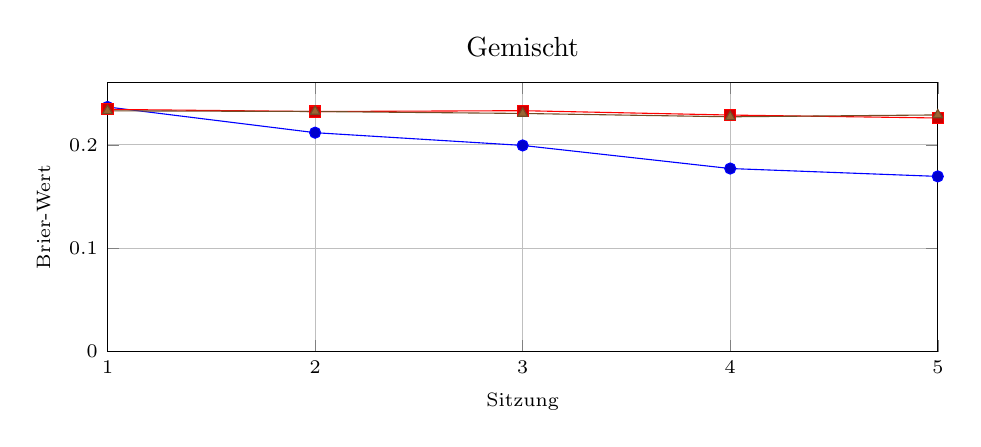
\begin{tikzpicture}
\begin{axis}[width=\linewidth,height=5cm,title={Gemischt},xlabel={Sitzung},ylabel={Brier-Wert},xmin=1,xmax=5,xtick={1,...,5},ymin=0,grid=major,tick label style={font=\scriptsize},label style={font=\scriptsize}]
\addplot+[mark=*] coordinates {(1,0.23659261645741989) (2,0.2117290140448366) (3,0.19939482043392354) (4,0.17706689338909865) (5,0.16946092824650208)};
\addplot+[mark=square*] coordinates {(1,0.23425022814843785) (2,0.23217843935351873) (3,0.2330022165635759) (4,0.22877644712011275) (5,0.2259276641329822)};
\addplot+[mark=triangle*] coordinates {(1,0.23285340846766617) (2,0.2322123472892886) (3,0.2303090635648175) (4,0.22708617735731604) (5,0.22889040472257885)};
\end{axis}
\end{tikzpicture}
\end{minipage}\par\medskip
\begin{minipage}{0.48\textwidth}\centering
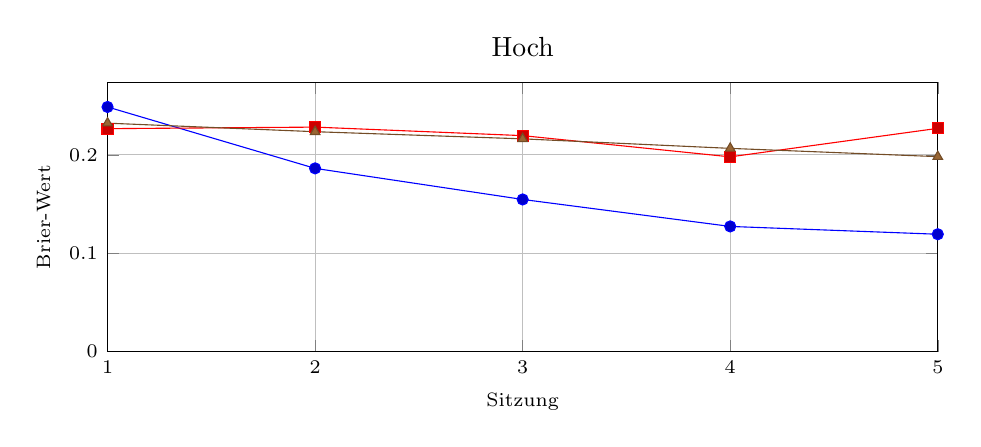
\begin{tikzpicture}
\begin{axis}[width=\linewidth,height=5cm,title={Hoch},xlabel={Sitzung},ylabel={Brier-Wert},xmin=1,xmax=5,xtick={1,...,5},ymin=0,grid=major,tick label style={font=\scriptsize},label style={font=\scriptsize}]
\addplot+[mark=*] coordinates {(1,0.2486125466728814) (2,0.18622587094282975) (3,0.15464667350259498) (4,0.12723364398659576) (5,0.11930203829748738)};
\addplot+[mark=square*] coordinates {(1,0.2265662320386342) (2,0.22814723889462907) (3,0.21948839492136155) (4,0.19792579881781353) (5,0.22689122448092375)};
\addplot+[mark=triangle*] coordinates {(1,0.23216212089000327) (2,0.22348240630387678) (3,0.21622082045548371) (4,0.2065396558554648) (5,0.19814060852529122)};
\end{axis}
\end{tikzpicture}
\end{minipage}\hfill
\begin{minipage}{0.48\textwidth}\centering
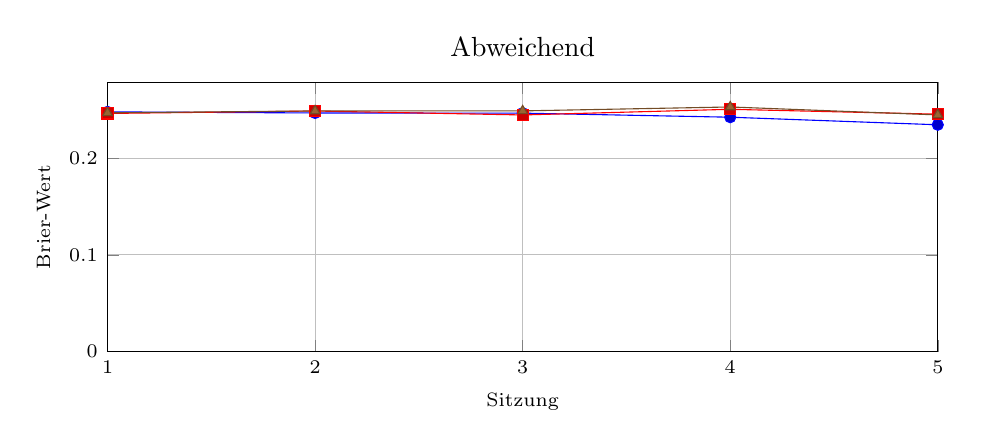
\begin{tikzpicture}
\begin{axis}[width=\linewidth,height=5cm,title={Abweichend},xlabel={Sitzung},ylabel={Brier-Wert},xmin=1,xmax=5,xtick={1,...,5},ymin=0,grid=major,tick label style={font=\scriptsize},label style={font=\scriptsize}]
\addplot+[mark=*] coordinates {(1,0.24782296154360683) (2,0.24669535762636016) (3,0.24651617661940498) (4,0.24230566095163297) (5,0.2344835494682723)};
\addplot+[mark=square*] coordinates {(1,0.2461961728887983) (2,0.24872285712198064) (3,0.244636232355797) (4,0.25047448127967814) (5,0.24544104004669545)};
\addplot+[mark=triangle*] coordinates {(1,0.24681799485683492) (2,0.24878555609583355) (3,0.24882937603988942) (4,0.25289364915321627) (5,0.24467048410844935)};
\end{axis}
\end{tikzpicture}
\end{minipage}\par\medskip
\par\smallskip\footnotesize Blau/Kreise: Zufall; Rot/Quadrate: Bewertungen und Lernstand; Braun/Dreiecke: Informationsgewinn.}
\newcommand{\EvaluationNeedPlot}{%
\begin{minipage}{0.48\textwidth}\centering
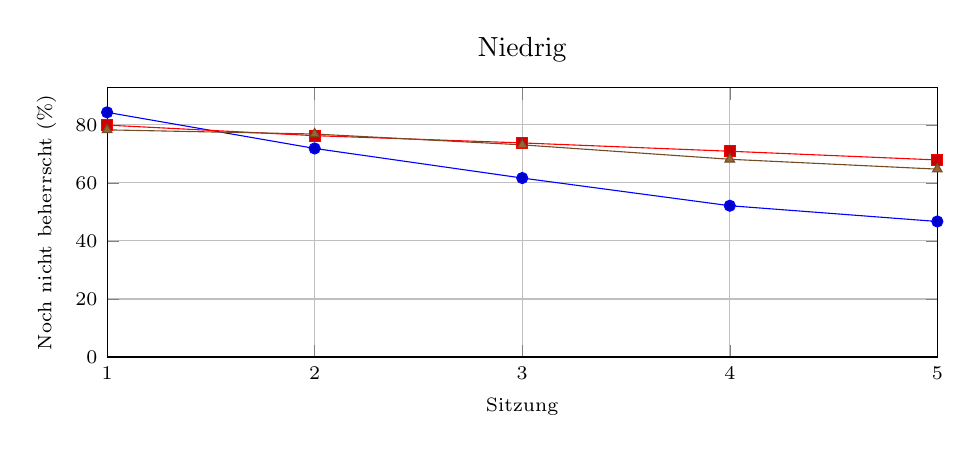
\begin{tikzpicture}
\begin{axis}[width=\linewidth,height=5cm,title={Niedrig},xlabel={Sitzung},ylabel={Noch nicht beherrscht (\%)},xmin=1,xmax=5,xtick={1,...,5},ymin=0,grid=major,tick label style={font=\scriptsize},label style={font=\scriptsize}]
\addplot+[mark=*] coordinates {(1,84.29999999999993) (2,71.86666666666667) (3,61.66666666666668) (4,52.13333333333333) (5,46.69999999999999)};
\addplot+[mark=square*] coordinates {(1,79.89999999999998) (2,76.26666666666664) (3,73.76666666666667) (4,70.89999999999999) (5,67.90000000000002)};
\addplot+[mark=triangle*] coordinates {(1,78.26666666666661) (2,76.83333333333331) (3,73.1) (4,68.13333333333337) (5,64.73333333333336)};
\end{axis}
\end{tikzpicture}
\end{minipage}\hfill
\begin{minipage}{0.48\textwidth}\centering
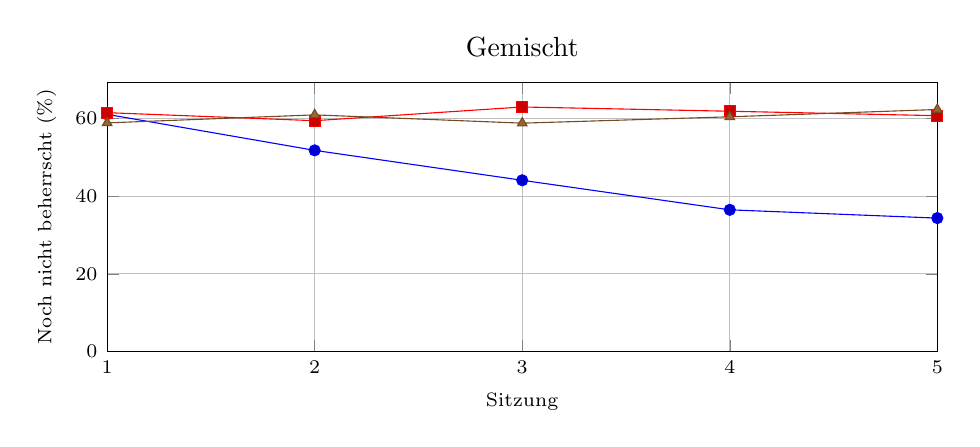
\begin{tikzpicture}
\begin{axis}[width=\linewidth,height=5cm,title={Gemischt},xlabel={Sitzung},ylabel={Noch nicht beherrscht (\%)},xmin=1,xmax=5,xtick={1,...,5},ymin=0,grid=major,tick label style={font=\scriptsize},label style={font=\scriptsize}]
\addplot+[mark=*] coordinates {(1,61.066666666666706) (2,51.800000000000004) (3,44.09999999999999) (4,36.49999999999999) (5,34.366666666666674)};
\addplot+[mark=square*] coordinates {(1,61.5) (2,59.43333333333336) (3,62.96666666666668) (4,61.86666666666669) (5,60.72194188619973)};
\addplot+[mark=triangle*] coordinates {(1,58.86666666666668) (2,60.93333333333334) (3,58.80000000000003) (4,60.43333333333335) (5,62.317266922094504)};
\end{axis}
\end{tikzpicture}
\end{minipage}\par\medskip
\begin{minipage}{0.48\textwidth}\centering
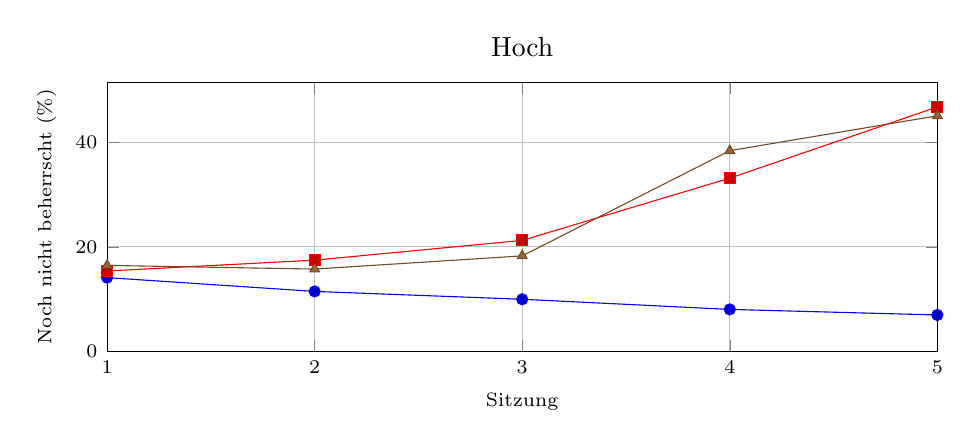
\begin{tikzpicture}
\begin{axis}[width=\linewidth,height=5cm,title={Hoch},xlabel={Sitzung},ylabel={Noch nicht beherrscht (\%)},xmin=1,xmax=5,xtick={1,...,5},ymin=0,grid=major,tick label style={font=\scriptsize},label style={font=\scriptsize}]
\addplot+[mark=*] coordinates {(1,14.133333333333315) (2,11.49999999999999) (3,9.999999999999995) (4,8.066666666666663) (5,6.9999999999999964)};
\addplot+[mark=square*] coordinates {(1,15.399999999999986) (2,17.466666666666654) (3,21.23563218390805) (4,33.11497488073324) (5,46.70843776106933)};
\addplot+[mark=triangle*] coordinates {(1,16.466666666666644) (2,15.766666666666648) (3,18.283678160919525) (4,38.36218458692412) (5,45.028583137135776)};
\end{axis}
\end{tikzpicture}
\end{minipage}\hfill
\begin{minipage}{0.48\textwidth}\centering
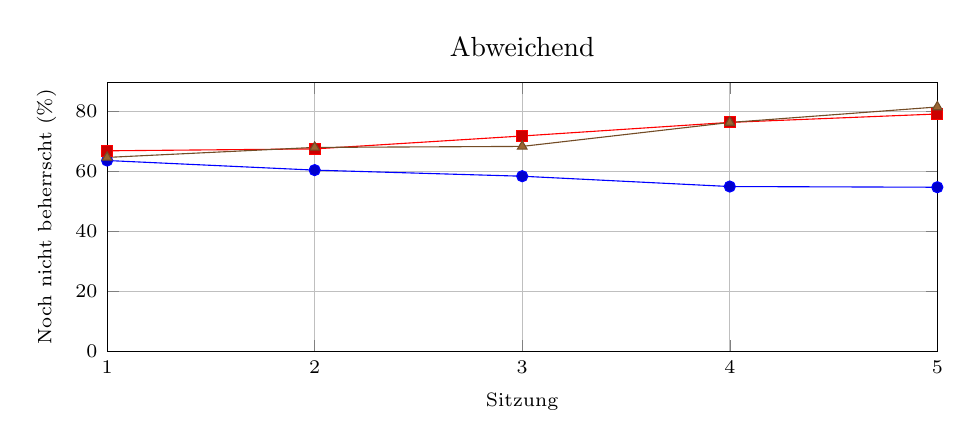
\begin{tikzpicture}
\begin{axis}[width=\linewidth,height=5cm,title={Abweichend},xlabel={Sitzung},ylabel={Noch nicht beherrscht (\%)},xmin=1,xmax=5,xtick={1,...,5},ymin=0,grid=major,tick label style={font=\scriptsize},label style={font=\scriptsize}]
\addplot+[mark=*] coordinates {(1,63.666666666666686) (2,60.46666666666668) (3,58.43333333333334) (4,55.00000000000003) (5,54.76666666666667)};
\addplot+[mark=square*] coordinates {(1,66.89999999999998) (2,67.53333333333333) (3,71.83333333333337) (4,76.36666666666667) (5,79.16666666666664)};
\addplot+[mark=triangle*] coordinates {(1,64.70000000000002) (2,68.03333333333335) (3,68.36666666666666) (4,76.3333333333333) (5,81.5025641025641)};
\end{axis}
\end{tikzpicture}
\end{minipage}\par\medskip
\par\smallskip\footnotesize Blau/Kreise: Zufall; Rot/Quadrate: Bewertungen und Lernstand; Braun/Dreiecke: Informationsgewinn.}
\newcommand{\EvaluationCoveragePlot}{%
\begin{minipage}{0.48\textwidth}\centering
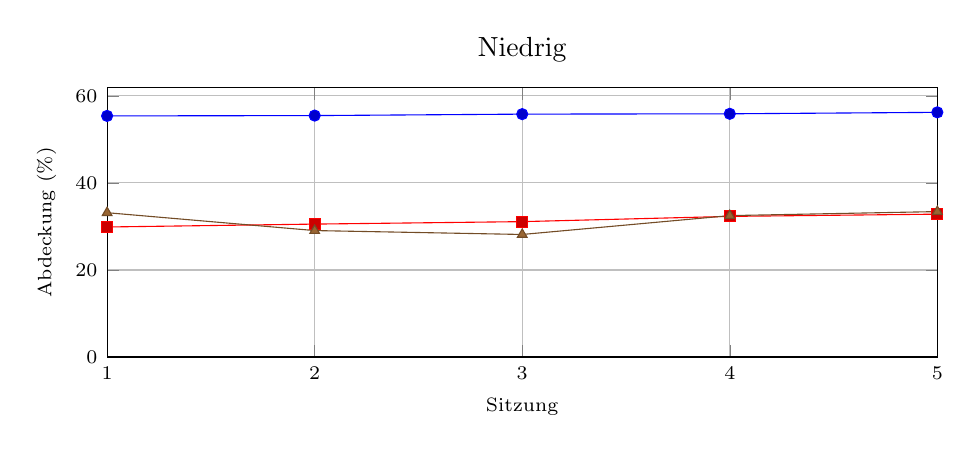
\begin{tikzpicture}
\begin{axis}[width=\linewidth,height=5cm,title={Niedrig},xlabel={Sitzung},ylabel={Abdeckung (\%)},xmin=1,xmax=5,xtick={1,...,5},ymin=0,grid=major,tick label style={font=\scriptsize},label style={font=\scriptsize}]
\addplot+[mark=*] coordinates {(1,55.38461538461538) (2,55.46153846153848) (3,55.794871794871824) (4,55.87179487179487) (5,56.20512820512822)};
\addplot+[mark=square*] coordinates {(1,29.871794871794837) (2,30.538461538461505) (3,31.102564102564063) (4,32.30769230769227) (5,32.82051282051278)};
\addplot+[mark=triangle*] coordinates {(1,33.15384615384611) (2,29.051282051282023) (3,28.153846153846118) (4,32.48717948717944) (5,33.41025641025637)};
\end{axis}
\end{tikzpicture}
\end{minipage}\hfill
\begin{minipage}{0.48\textwidth}\centering
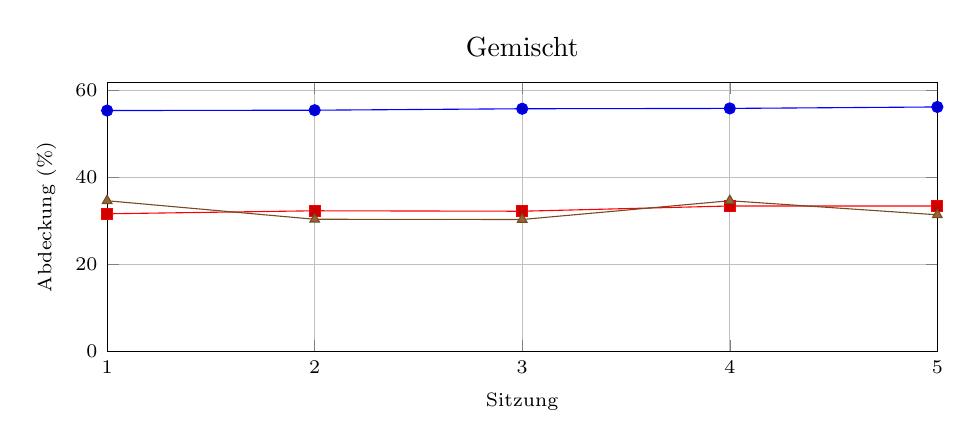
\begin{tikzpicture}
\begin{axis}[width=\linewidth,height=5cm,title={Gemischt},xlabel={Sitzung},ylabel={Abdeckung (\%)},xmin=1,xmax=5,xtick={1,...,5},ymin=0,grid=major,tick label style={font=\scriptsize},label style={font=\scriptsize}]
\addplot+[mark=*] coordinates {(1,55.38461538461538) (2,55.46153846153848) (3,55.794871794871824) (4,55.87179487179487) (5,56.20512820512822)};
\addplot+[mark=square*] coordinates {(1,31.666666666666625) (2,32.35897435897432) (3,32.25641025641021) (4,33.46153846153842) (5,33.461538461538424)};
\addplot+[mark=triangle*] coordinates {(1,34.66666666666662) (2,30.410256410256377) (3,30.358974358974322) (4,34.666666666666615) (5,31.43589743589739)};
\end{axis}
\end{tikzpicture}
\end{minipage}\par\medskip
\begin{minipage}{0.48\textwidth}\centering
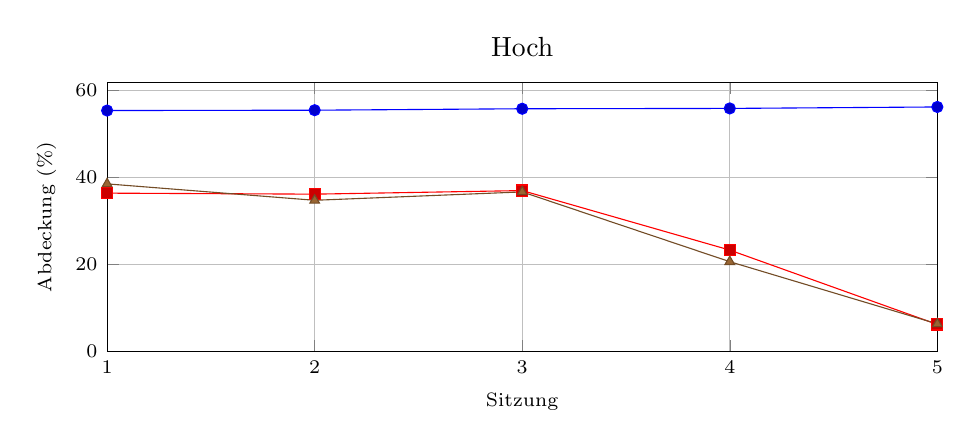
\begin{tikzpicture}
\begin{axis}[width=\linewidth,height=5cm,title={Hoch},xlabel={Sitzung},ylabel={Abdeckung (\%)},xmin=1,xmax=5,xtick={1,...,5},ymin=0,grid=major,tick label style={font=\scriptsize},label style={font=\scriptsize}]
\addplot+[mark=*] coordinates {(1,55.38461538461538) (2,55.46153846153848) (3,55.794871794871824) (4,55.87179487179487) (5,56.20512820512822)};
\addplot+[mark=square*] coordinates {(1,36.41025641025637) (2,36.17948717948713) (3,36.99999999999997) (4,23.333333333333304) (5,6.251800633823098)};
\addplot+[mark=triangle*] coordinates {(1,38.53846153846151) (2,34.76923076923073) (3,36.69230769230766) (4,20.66666666666664) (5,6.383547008547001)};
\end{axis}
\end{tikzpicture}
\end{minipage}\hfill
\begin{minipage}{0.48\textwidth}\centering
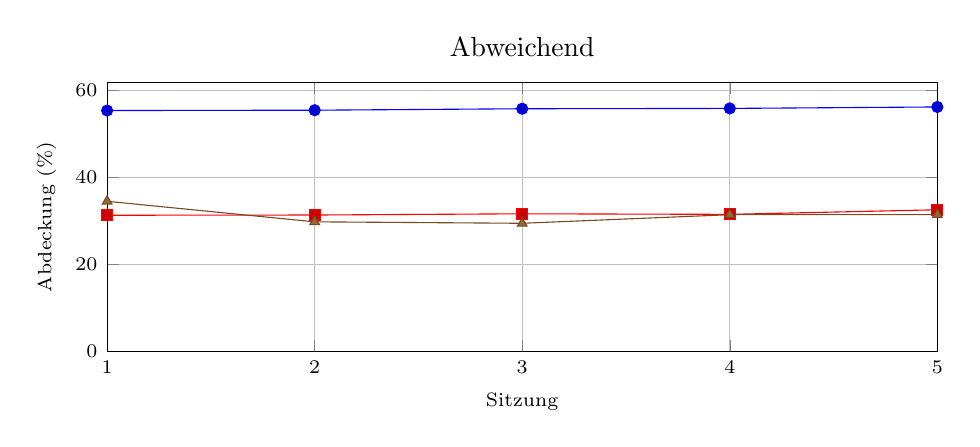
\begin{tikzpicture}
\begin{axis}[width=\linewidth,height=5cm,title={Abweichend},xlabel={Sitzung},ylabel={Abdeckung (\%)},xmin=1,xmax=5,xtick={1,...,5},ymin=0,grid=major,tick label style={font=\scriptsize},label style={font=\scriptsize}]
\addplot+[mark=*] coordinates {(1,55.38461538461538) (2,55.46153846153848) (3,55.794871794871824) (4,55.87179487179487) (5,56.20512820512822)};
\addplot+[mark=square*] coordinates {(1,31.33333333333329) (2,31.384615384615344) (3,31.666666666666625) (4,31.538461538461494) (5,32.58974358974355)};
\addplot+[mark=triangle*] coordinates {(1,34.5384615384615) (2,29.82051282051279) (3,29.48717948717945) (4,31.461538461538417) (5,31.487179487179446)};
\end{axis}
\end{tikzpicture}
\end{minipage}\par\medskip
\par\smallskip\footnotesize Blau/Kreise: Zufall; Rot/Quadrate: Bewertungen und Lernstand; Braun/Dreiecke: Informationsgewinn.}
\newcommand{\EvaluationEndpointTable}{%
\begin{tabular}{lrrrrrrrrr}
\hline
& \multicolumn{3}{c}{Zufall} & \multicolumn{3}{c}{Bewertungen + Lernstand} & \multicolumn{3}{c}{Informationsgewinn} \\
Situation & Aufgaben & Abdeckung & Brier & Aufgaben & Abdeckung & Brier & Aufgaben & Abdeckung & Brier \\
\hline
Niedrig & $150{,}0$ & $95{,}7$ & $0{,}1461$ & $150{,}0$ & $91{,}5$ & $0{,}1566$ & $150{,}0$ & $89{,}7$ & $0{,}1364$ \\
Gemischt & $150{,}0$ & $95{,}7$ & $0{,}1189$ & $149{,}8$ & $96{,}4$ & $0{,}1124$ & $149{,}8$ & $95{,}8$ & $0{,}1039$ \\
Hoch & $150{,}0$ & $95{,}7$ & $0{,}0615$ & $110{,}8$ & $100{,}0$ & $0{,}0216$ & $110{,}5$ & $100{,}0$ & $0{,}0216$ \\
Abweichend & $150{,}0$ & $95{,}7$ & $0{,}1756$ & $150{,}0$ & $93{,}0$ & $0{,}2387$ & $150{,}0$ & $90{,}8$ & $0{,}2215$ \\
\hline
\end{tabular}}


\chapter{Evaluation und Ergebnisse}
\label{chap:evaluation}

\section{Evaluationsdesign und Vorgehen}
\label{sec:evaluationsdesign}

Die leitende Fragestellung der Arbeit lautet, wie eine Lernplattform bisherige
Aufgabenbearbeitungen und Aufgaben-Kompetenz-Zuordnungen nutzen kann, um
individuelle Kompetenzstände zu schätzen und daraus nachvollziehbar passende
Folgeaufgaben auszuwählen. Die Evaluation untersucht diesen Zusammenhang anhand
simulierter Lernverläufe über bis zu fünf aufeinanderfolgende Sitzungen. Sie
betrachtet die Antwortvorhersagen des Lernstandsmodells, die Ausrichtung der
Auswahl auf noch nicht beherrschte Kompetenzen und die Kompetenzabdeckung.
Ergänzend wird der geschätzte Kompetenzstand mit dem bekannten simulierten
Zustand verglichen.

Die Untersuchung unterscheidet damit die Nutzung von Antworten für die
Lernstands\-schätzung von der Nutzung dieser Schätzung für die Aufgabenauswahl.
Eine gute Antwortvorhersage belegt nicht automatisch eine passende Auswahl.
Ebenso bedeutet eine häufige Auswahl noch nicht beherrschter Kompetenzen
nicht automatisch einen höheren Lernerfolg. Die Nachvollziehbarkeit wird an
einem konkreten Ablauf erläutert; ob reale Lernende die Auswahlgründe verstehen,
wird nicht durch eine Nutzerstudie untersucht.

Simulationen ermöglichen die kontrollierte Untersuchung von Verfahren für
intelligente Tutorsysteme \cite{vanlehn1994applications}. Hier sind insbesondere
die verborgenen Kompetenzzustände bekannt, die der Auswahlalgorithmus selbst
nicht beobachten kann. Die Ergebnisse gelten jedoch nur für die festgelegten
Annahmen und ersetzen keine Untersuchung mit realen Studierenden.

\subsection{Annahmen zur Simulation}

Für jede Kompetenz besitzt der simulierte Lernende einen binären Zustand:
beherrscht oder noch nicht beherrscht. Antworten und Lernübergänge werden
nach einem BKT-basierten Modell erzeugt \cite{corbett1994knowledge}.
Bei beherrschter Kompetenz kann ein Flüchtigkeitsfehler auftreten; bei
noch nicht beherrschter Kompetenz ist eine richtige Antwort durch Raten
möglich. Erst nach der Antwort kann eine noch nicht beherrschte Kompetenz
mit der angegebenen Lernrate in den beherrschten Zustand übergehen.
Vergessen, zeitliche Pausenwirkungen und aufgabenspezifische Erinnerung
werden nicht modelliert. Die verborgenen Kompetenzzustände entwickeln
sich unabhängig voneinander.

\begin{table}[htbp]
  \centering
  \small
  \begin{tabular}{lcccc}
    \hline
    Situation & Anfangskenntnis & Lernrate & Raten & Flüchtigkeitsfehler \\
    \hline
    Vorwissen niedrig & 0{,}10 & 0{,}18 & 0{,}20 & 0{,}10 \\
    Vorwissen gemischt & 0{,}35 & 0{,}18 & 0{,}20 & 0{,}10 \\
    Vorwissen hoch & 0{,}85 & 0{,}18 & 0{,}20 & 0{,}10 \\
    Abweichendes Lernverhalten & 0{,}35 & 0{,}05 & 0{,}30 & 0{,}20 \\
    \hline
  \end{tabular}
  \caption{Wahrscheinlichkeiten der vier simulierten Lernsituationen.
    Die Anfangskenntnis bestimmt den Zustand vor der ersten Sitzung.}
  \label{tab:szenarien}
\end{table}

Die Modellparameter des Algorithmus bleiben in allen Situationen gleich:
Anfangsschätzung $0{,}35$, Lernrate $0{,}18$, Ratewahrscheinlichkeit
$0{,}20$ und Flüchtigkeitsfehler $0{,}10$. Insbesondere wird das Modell
nicht an die Situation mit abweichendem Lernverhalten angepasst.
Die adaptiven Verfahren berücksichtigen hinterlegte Voraussetzungen bei
der Auswahl einer neuen Zielkompetenz. Diese Voraussetzungen beeinflussen
jedoch nicht den simulierten Antwort- oder Lernprozess.

\subsection{Der Beispielbestand der Plattform}

Die Untersuchung verwendet den Beispielbestand der Plattform. Seine
fachliche Grundlage bilden ausgewählte Inhalte der Vorlesungsfolien zum
Modul \emph{Datenbanksysteme} von Prof.\ Dr.\ habil.\ Markus Siepermann
an der Technischen Hochschule Mittelhessen
\cite{siepermannDatenbanksystemeFolien}. Die Kompetenzen und Aufgaben
wurden mit GPT-5 erstellt und vom Verfasser auf inhaltliche Plausibilität
durchgesehen. Sie dienen als vorläufige Entwicklungs- und Testdaten,
nicht als abschließend validierter Fragenkatalog.

Der Bestand enthält 48 Kompetenzen und 147 Aufgaben. Die fünf Aufgabentypen
sind Einfachauswahl, Mehrfachauswahl, Matrixaufgaben, Zuordnungsaufgaben und
Lückentextaufgaben. Für die Simulation werden nur Aufgaben mit genau einer
erforderlichen Kompetenz berücksichtigt, die nicht von der Auswahl
ausgeschlossen sind. Dadurch verbleiben 146 Aufgaben zu 39 Kompetenzen.
Die Zuordnung bestimmt, welcher verborgene Kompetenzzustand für die
Antworterzeugung verwendet und welche Schätzung nach der Antwort aktualisiert
wird. Die Simulation untersucht somit den binären Ein-Kompetenz-Fall,
nicht die vollständige Bewertung aller Aufgabenformate.

Die Aufgabeninhalte und ihre Schwierigkeit verändern die simulierte
Antwortwahrscheinlichkeit nicht. Schwierigkeit wird zwar von den adaptiven
Verfahren zur Auswahl einer Aufgabe herangezogen, ihre didaktische Wirkung
kann mit diesem Antwortmodell aber nicht geprüft werden. Eine in der
Simulation richtige Antwort bedeutet daher nicht, dass der konkrete
Aufgabentext von einer realen Person gelöst wurde.

\subsection{Antwortwahrscheinlichkeit und Lernstandsschätzung}

Der Algorithmus beobachtet nicht den verborgenen Kompetenzzustand, sondern
nur die simulierte Antwort. Aus der geschätzten Beherrschungswahrscheinlichkeit
$p$ berechnet er die Wahrscheinlichkeit einer richtigen Antwort als
$p(1-s)+(1-p)g$, wobei $s$ die Flüchtigkeitsfehler- und $g$ die
Ratewahrscheinlichkeit bezeichnet. Vor der ersten Sitzung ergibt sich:
\[
  0{,}35\cdot0{,}90+0{,}65\cdot0{,}20=0{,}445.
\]
Die Anfangsvorhersage beträgt damit $44{,}5\%$. Sie ist weder eine
erreichte Punktzahl noch die Beherrschungswahrscheinlichkeit selbst.
Nach einer Antwort aktualisiert der Algorithmus die Kompetenzschätzung
mit dem BKT-Posterior und dem anschließenden Lernübergang.

Ein simulierter Lernender beantwortet eine Aufgabe bei beherrschter
Kompetenz mit Wahrscheinlichkeit $0{,}90$ und sonst mit Wahrscheinlichkeit
$0{,}20$ richtig. Im abweichenden Szenario betragen diese Werte $0{,}80$
beziehungsweise $0{,}30$. Der Algorithmus verwendet dort weiterhin seine
unveränderten Modellannahmen.

\subsection{Verglichene Auswahlverfahren}

\begin{description}
  \item[Zufällige Auswahl:] Gleichverteilte Auswahl einer innerhalb der
    Sitzung noch nicht gestellten, geeigneten Aufgabe. Lernstand,
    Aufgabenschwierigkeit und Voraussetzungen bestimmen diese Wahl nicht.
  \item[Bewertungen und Lernstand:] Die Wahl einer neuen Zielkompetenz
    gewichtet wenige bisherige Bewertungen und einen niedrigen geschätzten
    Lernstand stärker. Anschließend wird eine Aufgabe für diese Kompetenz
    anhand der implementierten Schwierigkeits- und Utility-Heuristiken
    ausgewählt.
  \item[Informationsgewinn:] Die Wahl einer neuen Zielkompetenz richtet
    sich nach dem höchsten erwarteten Informationsgewinn einer weiteren
    binären Antwort. Die anschließende Aufgabenwahl verwendet dieselben
    Heuristiken wie das andere adaptive Verfahren.
\end{description}

Die adaptiven Verfahren behalten die bestehende Fokusphase bei:
Eine ausgewählte Kompetenz kann bis zu drei Aufgaben hintereinander
behandelt werden, sofern sie weiter Evidenz benötigt und geeignete
Aufgaben verfügbar sind. Die Kompetenzstrategie wird deshalb nicht vor
jeder Aufgabe unabhängig neu ausgeführt. Alle drei Verfahren verwenden
dasselbe Lernstandsmodell und dieselben Einstellungen für Aufgabenlimit
und Evidenzkriterium. Der Vergleich betrifft die vollständigen
Auswahlverfahren, nicht die isolierte Wirkung eines einzelnen Faktors.

\subsection{Umfang und Kennzahlen der Auswertung}

Für jede Kombination aus vier Situationen und drei Verfahren werden
100 Lernverläufe mit den Seeds 1 bis 100 berechnet. Jeder der insgesamt
1\,200 Lernverläufe umfasst bis zu fünf Sitzungen mit jeweils höchstens
30 Aufgaben. Damit werden nicht nur die ersten Antworten, sondern auch
die Auswahl auf Grundlage bereits aufgebauter Evidenz untersucht.
Die Zahl von fünf Sitzungen ist ein festgelegter Versuchsrahmen,
keine empirisch begründete optimale Trainingsdauer.
Das Auswertungsskript berechnet zusätzlich einen synthetischen
Kontrollbestand mit zehn Kompetenzen und je acht Aufgaben.
Die in diesem Kapitel berichteten Tabellen, Abbildungen und
Sitzungszahlen beziehen sich ausschließlich auf den Plattformbestand.

Zwischen den Sitzungen werden der simulierte Kompetenzzustand, die
geschätzten Beherrschungswahrscheinlichkeiten und die Bewertungszahlen
unverändert fortgeführt. Auch die Zufallsquellen laufen weiter. Neu
beginnen nur sitzungsbezogene Angaben wie Aufgabenhistorie, Fokusphase
und Ausschlüsse. Aufgaben dürfen in einer späteren Sitzung erneut
vorkommen, innerhalb einer Sitzung jedoch nicht. Die erneute Bearbeitung
verwendet dasselbe probabilistische Kompetenzmodell; das Erinnern einer
bereits gesehenen Lösung wird nicht simuliert.

Diese direkte Zustandsfortführung ist eine kontrollierte
Simulationsannahme. Sie ist keine vollständige Nachbildung des
Anwendungsstarts mit erneutem Einlesen und gegebenenfalls zeitlicher
Abschwächung historischer Antworten. Zwischen den Sitzungen wird kein
zusätzlicher Lernübergang allein durch den Sitzungswechsel ausgeführt.
Erfüllt der gesamte geeignete Kompetenzbestand beim nächsten
Sitzungsstart bereits das Evidenzkriterium, endet der Lernverlauf.
Ein Sitzungsende mangels noch auswählbarer Aufgaben kann dagegen durch
eine neue Sitzung mit erneut freigegebenen Aufgaben fortgesetzt werden.

Die Zufallsquellen für Auswahl und simulierte Lernende sind getrennt.
Bei gleichem Seed beginnen die Verfahren mit denselben verborgenen
Zuständen und denselben kompetenzbezogenen Zufallsfolgen. Da sie andere
Kompetenzen auswählen, entwickeln sich die Lernverläufe anschließend
unterschiedlich.

Die Vorhersagegüte wird mit Brier-Wert und Log-Loss bewertet
\cite{brier1950verification,pelanek2015metrics}. Für jede Antwort wird die
Vorhersage vor ihrer Verarbeitung gespeichert. Als Referenz wird die
feste Anfangsvorhersage von $44{,}5\%$ auf denselben Antworten ausgewertet.
Kleinere Werte bedeuten bessere Vorhersagen. Da die Verfahren
unterschiedliche Aufgaben auswählen, sind ihre Antwortvorhersagewerte
kein Vergleich auf identischen Antworten.

Für die Auswahl wird der Anteil der Aufgaben erfasst, deren Zielkompetenz
zum Auswahlzeitpunkt tatsächlich noch nicht beherrscht war. Die
Kompetenzabdeckung bezeichnet den Anteil der 39 Kompetenzen, die in der
jeweiligen Sitzung mindestens einmal vorkamen. Ergänzend wird die
Genauigkeit des gesamten geschätzten Kompetenzprofils mit dem mittleren
quadratischen Abstand zwischen geschätzter Beherrschungswahrscheinlichkeit
und binärem simuliertem Zustand bewertet.

Zunächst wird jede Kennzahl pro Sitzung berechnet; anschließend werden
Mittelwert und Stichprobenstandardabweichung über die Lernverläufe
zusammengefasst. Die bis zu fünf Sitzungen einer Person gelten nicht als
unabhängige Wiederholungen. Bei vorzeitig beendeten Lernverläufen enthalten
spätere Sitzungswerte nur die noch aktiven Verläufe. Abweichende Fallzahlen
werden daher als Index $n$ ausgewiesen; ein Strich bedeutet, dass keine
Sitzung mehr stattfand. Die abschließende Gesamtauswertung verwendet
dagegen den letzten Zustand jedes der 100 Lernverläufe einer Kombination,
auch wenn dieser bereits vor der fünften Sitzung erreicht wurde.

\section{Beispiel: Aktualisierung der Lernstandsschätzung}
\label{sec:exemplarischer-ablauf}

Das Beispiel zeigt die ersten fünf Aufgaben des Lernverlaufs mit Seed 1,
gemischtem Vorwissen und Auswahl nach erwartetem Informationsgewinn.
Es erläutert die Verarbeitung einer Antwort, nicht die allgemeine
Überlegenheit eines Verfahrens.

\begin{table}[htbp]
  \centering
  \small
  \begin{tabular}{rp{6cm}cc}
    \hline
    Aufgabe & Zielkompetenz & Antwortvorhersage & Antwort \\
    \hline
    1 & Daten, Information und Wissen & 45\% & falsch \\
    2 & Datenhierarchie & 45\% & falsch \\
    3 & Datentypen und Datenkategorien & 45\% & richtig \\
    4 & Datentypen und Datenkategorien & 73\% & falsch \\
    5 & Eigenschaften von Information & 45\% & richtig \\
    \hline
  \end{tabular}
  \caption{Erste fünf Aufgaben der ersten Sitzung. Die Antwortvorhersage
    wird jeweils vor Verarbeitung der angezeigten Antwort bestimmt.}
  \label{tab:beispiel-sitzung}
\end{table}

Bei Aufgabe 3 beherrschte der simulierte Lernende die Kompetenz noch
nicht, antwortete jedoch richtig. Der Algorithmus kennt diesen Zustand
nicht und erhöht aufgrund der Antwort seine Beherrschungsschätzung von
$0{,}35$ auf rund $0{,}76$. Daraus ergibt sich vor Aufgabe 4 eine
Antwortvorhersage von rund $73\%$. Die folgende falsche Antwort ist kein
Widerspruch, weil die Vorhersage eine Wahrscheinlichkeit und keine
Gewissheit ausdrückt. Eine richtige Antwort liefert Evidenz, beweist aber
nicht die Beherrschung einer Kompetenz.

Die Aufgaben-Kompetenz-Zuordnung stellt dabei die Verbindung zwischen
Antwort und Schätzung her: Die beiden Aufgaben zu Datentypen verändern
die Schätzung derselben Kompetenz, nicht pauschal die Schätzungen aller
Kompetenzen. Bei Aufgabe 4 wird die bereits ausgewählte Kompetenz
innerhalb der Fokusphase erneut behandelt. Der Auswahlgrund ist hier
also nicht zwingend eine neue globale Maximierung des Informationsgewinns,
sondern die Kombination aus Kompetenzstrategie und Fokusregel.

In späteren Sitzungen werden die erreichten Kompetenzschätzungen und
Bewertungszahlen weiterverwendet. Die Auswahl beginnt dann nicht erneut
bei identischen Anfangswerten. Das Beispiel macht den Datenfluss von
Aufgabe über Kompetenzzuordnung und Antwort zu Schätzung und Folgeaufgabe
nachvollziehbar. Es ist jedoch weder ein Nutzertest der Verständlichkeit
noch ein Beleg für die fachliche Qualität jedes Aufgabentextes.

\section{Vorhersage der Antworten}
\label{sec:evaluation-lernstand}

Die Tabellen zeigen die Vorhersagewerte getrennt nach Situation,
Auswahlverfahren und Sitzungsnummer. Je Zelle stehen Mittelwert und
Standardabweichung des Lernstandsmodells. In Klammern folgt der Mittelwert
der festen Anfangsvorhersage auf denselben Antworten. Die Sitzungsnummer
kennzeichnet den Verlauf derselben simulierten Lernenden; sie bezeichnet
keine fünf unabhängig neu gestarteten Gruppen.

\begin{table}[htbp]
  \centering
  \resizebox{\textwidth}{!}{\EvaluationBrierTable}
  \caption{Brier-Wert der Antwortvorhersagen über bis zu fünf Sitzungen.
    In Klammern: feste Vorhersage von $44{,}5\%$. Ein Index $n$ weist auf
    eine von 100 abweichende Fallzahl hin.}
  \label{tab:brier}
\end{table}

\begin{table}[htbp]
  \centering
  \resizebox{\textwidth}{!}{\EvaluationLogLossTable}
  \caption{Log-Loss der Antwortvorhersagen. Darstellung und Referenz
    entsprechen Tabelle~\ref{tab:brier}.}
  \label{tab:logloss}
\end{table}

\begin{figure}[htbp]
  \centering
  \EvaluationBrierPlot
  \caption{Verlauf des Brier-Werts nach Situation. Die Kurven beziehen
    sich auf die jeweils noch aktiven Lernverläufe und auf unterschiedliche
    ausgewählte Antworten; sie zeigen keinen Lernerfolgsvergleich.}
  \label{fig:brier}
\end{figure}

In der ersten Sitzung liegen die Vorhersagewerte aller Verfahren in
allen Situationen unter denen der festen Anfangsvorhersage. Dies
bestätigt, dass die Aktualisierung anhand der bisherigen Antworten in
diesem Kaltstartvergleich nützliche Informationen für die Antwortvorhersage
liefert. Daraus folgt jedoch nicht, dass die adaptive Auswahl besser als
Zufall ist: Auch die Zufallsauswahl verwendet dasselbe aktualisierte
Lernstandsmodell.

In späteren Sitzungen muss zusätzlich berücksichtigt werden, welche
Aufgaben die Verfahren noch stellen. Eine Auswahl kann sich auf
unsichere oder noch nicht beherrschte Kompetenzen konzentrieren und
damit andere Antwortfolgen erhalten als ein breit auswählendes
Verfahren. Ein niedrigerer Vorhersagefehler auf diesen unterschiedlichen
Antworten ist deshalb kein isolierter Qualitätsnachweis der
Auswahlstrategie. Insbesondere ist nicht vorauszusetzen, dass die
aktualisierte Schätzung in jeder späteren Situation besser als die feste
Referenz bleibt; dies wird für jede Sitzung gesondert ausgewiesen.

Dies zeigt sich im Szenario mit abweichendem Lernverhalten besonders
deutlich: In der fünften Sitzung beträgt der Brier-Wert bei der
Gewichtung nach Bewertungen und Lernstand $0{,}2454$ gegenüber $0{,}2443$
für die feste Referenz. Beim Informationsgewinnverfahren stehen
$0{,}2447$ dem Referenzwert $0{,}2404$ gegenüber. Eine fortgeführte
Historie gleicht unpassende Modellannahmen somit nicht automatisch aus.

\section{Auswahlverhalten und Kompetenzabdeckung}
\label{sec:evaluation-auswahl}

Für die Frage nach passenden Folgeaufgaben wird untersucht, ob die
Auswahl auf tatsächlich noch nicht beherrschte Kompetenzen fällt.
Tabelle~\ref{tab:selection-need} berichtet deren Anteil an den Aufgaben
einer Sitzung. Die Mittelwerte und Standardabweichungen sind in Prozent
beziehungsweise Prozentpunkten angegeben.

\begin{table}[htbp]
  \centering
  \resizebox{\textwidth}{!}{\EvaluationNeedTable}
  \caption{Anteil der Aufgaben mit noch nicht beherrschter Zielkompetenz
    zum Auswahlzeitpunkt. Ein größerer Wert zeigt häufigere Auswahl
    bestehenden simulierten Lernbedarfs, nicht unmittelbar mehr Lernen.}
  \label{tab:selection-need}
\end{table}

\begin{figure}[htbp]
  \centering
  \EvaluationNeedPlot
  \caption{Ausrichtung auf noch nicht beherrschte Kompetenzen im
    Sitzungsverlauf. Spätere Werte umfassen nur noch aktive Lernverläufe.}
  \label{fig:selection-need}
\end{figure}

Bei gemischtem Vorwissen ist der Unterschied in der ersten Sitzung
noch gering: $61{,}1\%$ der zufällig ausgewählten Aufgaben betreffen
noch nicht beherrschte Kompetenzen, gegenüber $61{,}5\%$ bei der
Gewichtung nach Bewertungen und Lernstand und $58{,}9\%$ beim
Informationsgewinnverfahren. In der fünften Sitzung beträgt dieser
Anteil dagegen $34{,}4\%$ bei Zufall, $60{,}7\%$ bei der gewichteten
Auswahl und $62{,}3\%$ beim Informationsgewinnverfahren. Alle drei
Vergleichsgruppen umfassen hier weiterhin 100 Lernverläufe.
Der Abstand zur Zufallsauswahl beträgt damit $26{,}4$ beziehungsweise
$28{,}0$ Prozentpunkte. Die Verfahren weisen mit fortgeführter Evidenz
ein deutlich unterschiedliches Auswahlverhalten auf.

Auch bei niedrigem Vorwissen fallen in der fünften Sitzung bei den
adaptiven Verfahren häufiger Aufgaben auf noch nicht beherrschte
Kompetenzen: $67{,}9\%$ und $64{,}7\%$ gegenüber $46{,}7\%$ bei Zufall.
Im abweichenden Szenario sind es $79{,}2\%$ und $81{,}5\%$ gegenüber
$54{,}8\%$. Ein hoher Anteil zeigt dabei die Konzentration auf
verbleibenden Bedarf, nicht dessen erfolgreiche Beseitigung. Gerade
bei langsamen Lernübergängen können Kompetenzen trotz wiederholter
Bearbeitung noch nicht beherrscht sein. Die Kennzahl hängt folglich
auch vom durch die bisherige Auswahl entstandenen Kompetenzzustand ab.

Die Kompetenzabdeckung beschreibt dagegen, wie viele unterschiedliche
Kompetenzen in einer Sitzung behandelt werden. Ein hoher Anteil von
Aufgaben zu noch nicht beherrschten Kompetenzen kann mit einer geringen
Abdeckung einhergehen, wenn wiederholt dieselben Lücken bearbeitet werden.
Diese Kennzahlen beantworten daher verschiedene Fragen und dürfen nicht
als austauschbare Qualitätsmaße interpretiert werden.

\begin{figure}[htbp]
  \centering
  \EvaluationCoveragePlot
  \caption{Anteil der innerhalb einer Sitzung mindestens einmal
    behandelten Kompetenzen. Bezugsgröße sind die 39 geeigneten Kompetenzen.}
  \label{fig:coverage}
\end{figure}

Für die Gesamtbetrachtung fasst Tabelle~\ref{tab:trajectory-endpoints}
alle 100 Lernverläufe pro Kombination zusammen. Berichtet werden die
mittlere Gesamtzahl bearbeiteter Aufgaben, die kumulierte
Kompetenzabdeckung in Prozent und der Brier-Wert des Kompetenzprofils am
jeweiligen Ende des Lernverlaufs. Der Profilwert bewertet alle 39
Kompetenzen, einschließlich nicht bearbeiteter Kompetenzen. Er ist nicht
mit dem Brier-Wert der Antwortvorhersage gleichzusetzen.

\begin{table}[htbp]
  \centering
  \resizebox{\textwidth}{!}{\EvaluationEndpointTable}
  \caption{Gesamtbetrachtung bis einschließlich der fünften Sitzung.
    Pro Kombination gehen alle 100 Lernverläufe ein; bei früherem Ende
    wird deren letzter Zustand verwendet. Abdeckung in Prozent.
    Weniger Aufgaben bedeuten nicht automatisch mehr Effizienz, da das
    Evidenzkriterium keine nachgewiesene Kompetenzbeherrschung verlangt.}
  \label{tab:trajectory-endpoints}
\end{table}

Beim abschließenden Kompetenzprofil erreicht das Informationsgewinnverfahren
in den drei Situationen mit passenden Antwort- und Lernparametern
niedrigere Fehlerwerte als die Zufallsauswahl: $0{,}1364$ statt $0{,}1461$
bei niedrigem, $0{,}1039$ statt $0{,}1189$ bei gemischtem und $0{,}0216$
statt $0{,}0615$ bei hohem Vorwissen. Für die Gewichtung nach Bewertungen
und Lernstand gilt dieser Vorteil bei gemischtem und hohem, nicht aber
bei niedrigem Vorwissen. Im abweichenden Szenario sind dagegen beide
adaptiven Verfahren ungenauer als Zufall: $0{,}2387$ beziehungsweise
$0{,}2215$ gegenüber $0{,}1756$. Es handelt sich um deskriptive
Mittelwertvergleiche, nicht um nachgewiesene statistische Signifikanz.

Bei hohem Vorwissen bearbeiten die adaptiven Verfahren über den
gesamten Lernverlauf im Mittel rund 111 Aufgaben gegenüber 150 bei
Zufall und erreichen dabei eine kumulierte Abdeckung von $100\%$.
Die Zufallsauswahl erreicht $95{,}7\%$. Die geringere Aufgabenanzahl
darf jedoch nicht allein als effizienterer Abschluss interpretiert
werden: Sitzungen können auch enden, weil unter den bestehenden
Auswahlregeln keine weitere geeignete Aufgabe verfügbar ist.

Insgesamt wurden im Plattformbestand \EvaluationSessions{} Sitzungen mit
\EvaluationAnswers{} Antworten ausgeführt. Davon endeten
\EvaluationEvidenceEnds{} Sitzungen wegen des Evidenzkriteriums und
\EvaluationNoQuestionEnds{} mangels einer weiteren auswählbaren Aufgabe.
Die übrigen Sitzungen erreichten das Aufgabenlimit. Innerhalb einer
Sitzung sind Wiederholungen durch den Ausschluss bereits bearbeiteter
Aufgaben verhindert. Zwischen Sitzungen sind sie ausdrücklich zugelassen.
Gemessen wird die Zahl bearbeiteter Aufgaben, nicht die reale
Bearbeitungszeit.

\subsection{Zentrale Erkenntnisse und Grenzen}
\label{subsec:zentrale-erkenntnisse}

Die Evaluation beantwortet die Leitfrage auf der Ebene des implementierten
Datenflusses: Antworten werden über die Aufgaben-Kompetenz-Zuordnung einer
Kompetenz zugeordnet, ihre Schätzung wird aktualisiert und beeinflusst
zusammen mit Bewertungszahlen, Fokusphase und Auswahlstrategie die
Folgeaufgaben. Der mehrsitzige Versuchsaufbau untersucht diesen Ablauf
nicht nur im Kaltstart, sondern auch mit fortgeführter Evidenz.

Das zentrale positive Ergebnis liegt in der gezielteren Ausrichtung
späterer Folgeaufgaben auf noch nicht beherrschte Kompetenzen. Bei
gemischtem Vorwissen steigt der Abstand zur Zufallsauswahl in der
fünften Sitzung auf rund 26 bis 28 Prozentpunkte. Zusätzlich erreicht
das Informationsgewinnverfahren am Ende der mehrsitzigen Untersuchung
in allen drei Situationen mit passenden Antwort- und Lernparametern
ein genaueres Gesamtprofil als die Zufallsauswahl. Die Evaluation
zeigt damit einen konkreten Nutzen der implementierten adaptiven
Auswahl unter diesen Simulationsbedingungen, ohne eine allgemeine
Überlegenheit zu behaupten. Die schlechteren Profilwerte im
abweichenden Szenario verdeutlichen zugleich die Grenzen der
gewählten Modellannahmen.

Die Beurteilung des Nutzens muss dabei zwischen Antwortvorhersage,
Ausrichtung der Auswahl und Genauigkeit des Gesamtprofils unterscheiden.
Die Auswahl noch nicht beherrschter Kompetenzen ist ein Hinweis auf
gezielte Bearbeitung vorhandener Lücken. Sie ist aber kein Nachweis, dass
die ausgewählten Aufgaben einen größeren Lernzuwachs verursachen.
Der Vergleich des gesamten Kompetenzprofils berücksichtigt auch die
Breite der erhobenen Evidenz. Keines dieser Maße allein beantwortet
sämtliche Aspekte einer passenden Folgeaufgabe.

Die wissenschaftliche Aussage bleibt auf das simulierte Modell
beschränkt. Die Antworten wurden mit einem BKT-basierten Prozess erzeugt,
während die Plattform ebenfalls ein BKT-basiertes Modell zur Schätzung
verwendet. Der Bestand ist vorläufig, die Schwierigkeit wirkt nicht auf
Antworten oder Lernen, und wiederholte Aufgaben erzeugen keine besondere
Erinnerungswirkung. Die Fortführung der Zustände bildet zudem keine
zeitliche Abschwächung historischer Evidenz ab. Schließlich bedeutet ein
Ende wegen ausreichender Diagnoseevidenz nicht zwingend, dass sämtliche
Kompetenzen beherrscht werden. Aussagen über tatsächlichen Lernerfolg,
die Verständlichkeit der Auswahlgründe oder die Überlegenheit in realen
Lehrveranstaltungen erfordern deshalb weitere Untersuchungen.
